\documentclass[compress,dvips,xcolor={dvipsnames},t]{beamer}

\usepackage[english]{babel}
\usepackage{graphicx}
\usepackage{amssymb,amsmath}
\usepackage{xspace}

\renewcommand{\refname}{}
\newcommand\ASN{\textsf{ASN.1}\xspace}
\newcommand\Cpp{\mbox{\textsf{C} \hspace*{-2.5mm} \raise 0.7mm \hbox 
{${\scriptscriptstyle \textsf{++}}$}}\xspace}

\title{Teaching and research plans}
\author{Christian Rinderknecht}
\date{1st November 2012}

\begin{document}

\frame{\maketitle}

\begin{frame}
\frametitle{Teaching}

\begin{itemize}

  \item All kinds of computer programming, in particular, functional
  languages (OCaml, Erlang, XSLT, Haskell etc.).

  \item Analysis and proofs of algorithms (formal methods).

  \item Compiler construction (automata theory, formal grammars etc.).

  \item Unix development tools: emacs, bash, make, perl, mercurial.

  \item Cutting edge: ePUB3 (HTML5+CSS+MathML+tablets/phones, under
    development).

\end{itemize}

\end{frame}


\begin{frame}
\frametitle{Research}

\emph{Abstract Syntax Notation One} (\ASN) is a standardised language
(ISO, ITU-T) for defining data types whose values may be exchanged
across a network between two, possibly heterogeneous peers.

\bigskip

It is used in network management, secure email, mobile telephony, wireless applications, Long Term Evolution (4G~LTE), electronic commerce, air traffic control, voice and video over the internet, digital certificates, radio paging, interactive television, financial service systems, biometrics, ATM transactions, call routing to local carriers (USA), plane take-offs and landings, Federal Express tracking network, Microsoft Internet Explorer, Outlook, databases (genetics, libraries), diagnostic monitoring systems (car factories), metro equipments etc.

\bigskip

\emph{Encoding rules} specify how to serialize an \ASN value.

\end{frame}

\begin{frame}
\frametitle{\ASN and the compilation chain}

\begin{center}
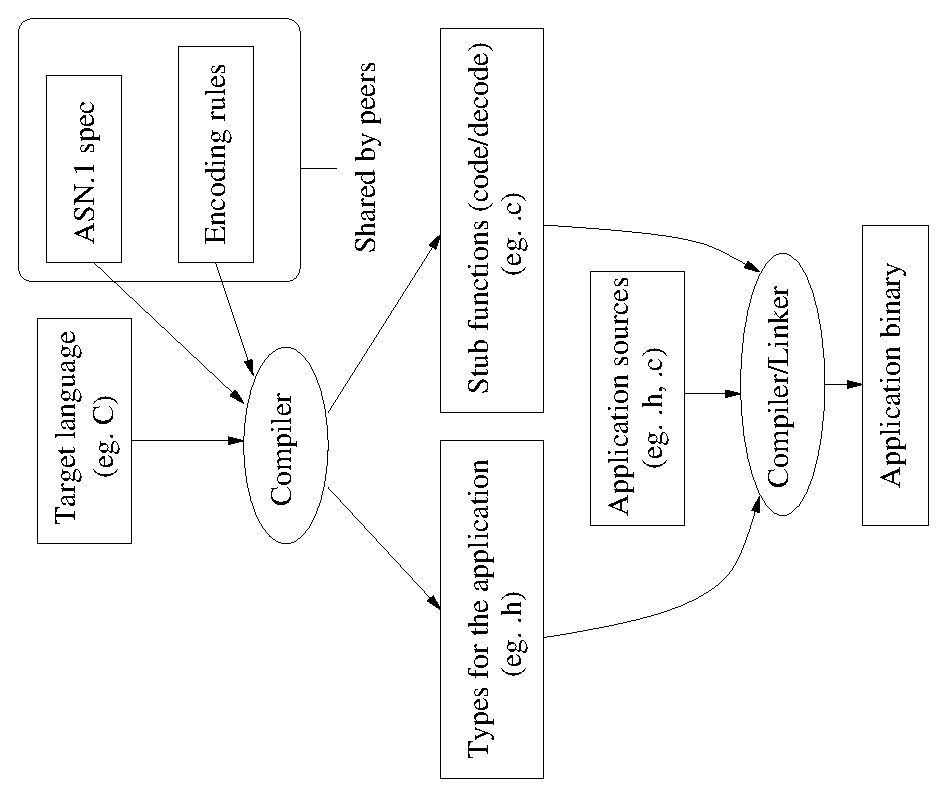
\includegraphics[scale=0.5]{compilation.eps}
\end{center}

\end{frame}

\begin{frame}
\frametitle{\ASN/BER and telecommunication}

\begin{center}
\includegraphics[scale=0.45]{model-1.eps}
\end{center}

\end{frame}

\begin{frame}
\frametitle{Issues}

\begin{enumerate}

  \item Specifications: huge (704 pages A4 10pt), complex (concepts
  mutually dependent).

  \item Syntax: large and ambiguous grammar, dynamic extensions.

  \item English cannot tell the meaning of all combinations of
    syntactical constructs.
  
  \item Types are value sets: subtypes yield general set constraints.

  \item Encoding only applies to a subset of \ASN.

  \item Decoding is unspecified.

  \item Dynamic checks in codecs (depending on the target programming
    language) are unspecified.

  \item Open source or free compilers: extremely rare, unmaintaned,
    fragile, without precise error reporting.

\end{enumerate}

\end{frame}

\begin{frame}
\frametitle{Issues in validation}

\ASN types are considered as sets of values, thus types must have at
least one (finite) value.

\bigskip

Because of the great expressivity of \ASN, the compilers are not
likely to fully check arbitrary combinations of subtyping
constraints!

\bigskip

Vendors' argument: ``This is hardly a real problem because
those critical specifications are rarely found in practice.''

\bigskip

My argument: ``Maintenance costs are always wildly underestimated. Why
not solve completely the problem, get a better product and save money
and time?''

\end{frame}


\begin{frame}
\frametitle{Problems}

\begin{enumerate}
  
  \item \label{finiteness} the types may have only infinite
        values:\\
        \texttt{T ::= SET \{a T\}};

  \item \label{type_conformance} some value declarations may be
        ill-typed:\\
        \texttt{v REAL ::= ""};

  \item \label{type_compatibility} especially, some value references
        may be ill-typed, as\\
        \texttt{a VisibleString ::= b}\\
        \texttt{b INTEGER ::= 0};

  \item \label{constraint_consistence} the subtype constraints may
        be inconsistent:\\
        \texttt{T ::= REAL (SIZE(7))};

  \item \label{subtype_non_emptyness} the subtypes may be empty, as\\
        \texttt{T ::= SET ((SIZE (1)) \symbol{94} (SIZE (2))) OF REAL};
        
  \item \label{solvability} the subtypes may have no value set:\\
        \texttt{T ::= REAL (ALL EXCEPT T)}. 

\end{enumerate}

\end{frame}

\begin{frame}
\frametitle{Problems (cont.)}

In other words, the issues to settle are respectively:

\begin{enumerate}

  \item the finiteness problem;
 
  \item the typechecking problem;

  \item the type compatibility problem;

  \item the constraint consistence problem;

  \item the non-emptyness problem;

  \item the solvability problem.

\end{enumerate}

\end{frame}

\begin{frame}
\frametitle{Analysis}

\begin{itemize}

  \item type compatibility $\subseteq$ typechecking;

  \item constraint consistence, non-emptyness $\subseteq$ solvability
        (the system is solved when we construct explicitly the values
        of each subtype);

  \item typechecking $\subseteq$ solvability:
\begin{tabular}{@{}rcl@{}}
   \texttt{y INTEGER (0..9) ::= 1}
   & $\rightarrow$ 
   & $\left\{
       \begin{tabular}{l} 
           \texttt{y A ::= 1} \\
           \texttt{A ::= INTEGER (0..9)} \\
           \texttt{B ::= A (y)}
        \end{tabular}
     \right.$
\end{tabular}
where \texttt{A}~and~\texttt{B} are fresh type references.

\end{itemize}

So, finiteness and solvability are enough to get a full validation of
\ASN.

\end{frame}

\begin{frame}
\frametitle{Two approaches}

Every \ASN specification is rewritten in a subset of same
expressiveness, with less syntactical constructs. Two strategies:

\begin{enumerate}

  \item Few preliminary rewrites, followed by a collection of set
  constraints, then fed to a generic constraint solver.

  \item Lots of preliminary rewrites, simple algorithms to check
    solvability. (This is like taking the previous method and
    interleave a dedicated solver with the syntactical rewrites.)

\end{enumerate}
Comparison:
\begin{enumerate}

\item Pros: modularity, less programming. Cons: constraints too
  general for off-the-shelf solvers.

  \item Pros: easy checking. Cons: heavily specialised, correctness
    hard to assess.

\end{enumerate}
We need to find a trade-off.

\end{frame}


\begin{frame}[containsverbatim]
\frametitle{Short presentation of \ASN}

\noindent
\textbf{Some basic types}
\begin{itemize}

  \item \verb+ok BOOLEAN ::= TRUE+

%%  \item The \texttt{NULL} type has only one value, also noted
%%        \texttt{NULL};

  \item 

\begin{verbatim} 
zero INTEGER ::= 0 
DayInTheYear ::= INTEGER {first(1), last(356)}
newYearsEve DayInTheYear ::= last
\end{verbatim}

  \item 
\begin{verbatim}
SynchroIndicator ::= ENUMERATED {serial,parallel}
synchro SynchroIndicator ::= serial
\end{verbatim}

  \item

\begin{verbatim}
pi REAL ::= 3.14159
micron REAL ::= {mantissa 1,base 10,exponent -6}
\end{verbatim}

  \item 

\begin{verbatim}
byte BIT STRING ::= 'OD'H  -- or '00001110'B
T ::= BIT STRING {msb(7), lsb(0)}
v T ::= {msb, lsb}  -- or '10000001'B
\end{verbatim}

%%  \item The \texttt{OCTET STRING} type is similar to the \texttt{BIT
%%        STRING} for eight-bit multiples strings.

%%  \item The \texttt{OBJECT IDENTIFIER} and \texttt{RELATIVE-OID} types
%%        aim at referencing other \ASN modules (a set of type
%%        and value declarations) at an international level, by means of
%%        a path in a standard tree.

  \item For historical reasons, there are many string types.

\end{itemize}

\end{frame}

\begin{frame}[containsverbatim]
\frametitle{Some constructed types}

The \texttt{SET} type corresponds to the record-like structures in
programming languages:
\begin{verbatim}
PersonInfo ::= SET {age INTEGER, married BOOLEAN}
i PersonInfo ::= {married TRUE, age 42}
\end{verbatim}
Some fields can be marked as optional or having a default value:
\begin{verbatim}
Point ::= SET {x REAL DEFAULT 0, y REAL DEFAULT 0}
origin Point ::= {}           -- or {x 0.0, y 0.0}
\end{verbatim}
A real example:
\begin{verbatim}
DataAcknowledgementTPDU ::= SET {
  destRef        Reference,
  yr-tu-nr       TPDUnumber,
  checkSum       CheckSum OPTIONAL,
  subSeqNr       SubSequenceNumber DEFAULT 0,
  flowControlCnf FlowControlConfirmation OPTIONAL}
\end{verbatim}

\end{frame}

\begin{frame}[containsverbatim]
\frametitle{Some constructed types (cont.)}

The \texttt{SET OF} type corresponds to the mathematical notion of
sets with repetition:
\begin{verbatim}
T ::= SET OF INTEGER
empty T ::= {}
small T ::= {7, 9, 1, 1, 3}
\end{verbatim}

\end{frame}

\begin{frame}[containsverbatim]
\frametitle{Some constructed types (cont.)}

The \texttt{CHOICE} type corresponds to a \textbf{union} in C.
\begin{verbatim}
T ::= CHOICE {x REAL, y BOOLEAN}
u T ::= x : 0.5
v T ::= y : FALSE
\end{verbatim}
The Protocol Data Units (PDU) are \texttt{CHOICE} types, because they
model all the possible queries and responses between two peers. A
\texttt{CHOICE} type may be recursive, like the other constructed
types. One real example (a Network Management Protocol) is:
\begin{verbatim}
CMISFilter ::= CHOICE {
  item  FilterItem,
  and   SET OF CMISFilter,
  or    SET OF CMISFilter,
  not   CMISFilter}
\end{verbatim}

\end{frame}

\begin{frame}[containsverbatim]
\frametitle{Some subtyping constraints}

\ASN offers a very involved subtyping paradigm consisting of
constraints upon recursive types, that restricts their corresponding
sets of values in a set-theoritic manner, but also in a structural
way.
\begin{itemize}

  \item \textbf{Interval Constraint}: the \texttt{INTEGER},
  \texttt{REAL} and (almost all) string types have totally ordered
  values, hence allowing interval definitions. For instance:

\begin{verbatim}
PositiveOrZeroInteger ::= INTEGER (0..MAX)
PositiveInteger ::= INTEGER (0<..MAX)
NegativeOrZeroInteger ::= INTEGER (MIN..0)
NegativeInteger ::= INTEGER (MIN..<0)
PositiveReal ::= REAL (0<..PLUS-INFINITY)
NegativeReal ::= REAL (MINUS-INFINITY..<0)
RealInterval ::= REAL (4e-5..1e-4)
\end{verbatim}
\end{itemize}

\end{frame}

\begin{frame}[containsverbatim]
\frametitle{Some subtyping constraints (cont.)}

\begin{itemize}

  \item \textbf{Value Constraint}: to restrict the set of values of a
  type to be a singleton:

\begin{verbatim}
Wednesday ::= Day (wednesday)
\end{verbatim}

  \item \textbf{Union Constraint}: the new subtype contains the values
  of the first subtype and of the second subtype (keyword
  \texttt{UNION} or symbol \texttt{|}):

\begin{verbatim}
Day ::= ENUMERATED {monday, tuesday, wednesday, 
              thursday, friday, saturday, sunday}
WeekEnd ::= Day (saturday | sunday)
\end{verbatim}

  \item \textbf{Alphabet Constraint}: the strings can be restricted to
  be built upon a given alphabet:

\begin{verbatim}
CapitalAndSmall ::= 
  IA5String (FROM ("A".."Z" | "a".."z"))
CapitalOrSmall ::= 
  IA5STring (FROM ("A".."Z") | FROM ("a".."z"))
\end{verbatim}

\end{itemize}

\end{frame}

\begin{frame}[containsverbatim]
\frametitle{Some subtyping constraints (cont.)}

\begin{itemize}

  \item \textbf{Size Constraint}: the values of string types may be
        constrained to a given sizes, introducing a constraint by the
        keyword \texttt{SIZE}:

\begin{verbatim}
Exactly31BitsString ::= BIT STRING (SIZE (31))
StringOf31BitsAtTheMost ::=
  BIT STRING (SIZE (0..31))
NonEmptyString ::= BIT STRING (SIZE (1..MAX))
\end{verbatim}

The size constraint can also apply to \texttt{SET OF} types. In that
case, the semantics is very different: the values of the types are
sets whose \emph{cardinals} are specified by the size constraint:

\begin{verbatim}
SetOf5Strings ::=
  SET (SIZE(5)) OF PrintableString
SetOfStringsOf5Char::=
  SET OF PrintableString (SIZE(5))
\end{verbatim}

\end{itemize}

\end{frame}

\begin{frame}[containsverbatim]
\frametitle{Some subtyping constraints (cont.)}

\begin{itemize}

  \item \textbf{Intersection Constraint}: the new subtype contains the
        values that belong to the two subtypes (keyword
        \texttt{INTERSECTION} or symbol \texttt{\symbol{94}}):

\begin{verbatim}
FrenchPhoneNumber ::= 
  NumericString (FROM ("0".."9") ^ SIZE (10))
\end{verbatim}

  \item \textbf{Inclusion Constraint}: to restrict a subtype to have
        only the values of a given subtype (optional keyword
        \texttt{INCLUDES}):

\begin{verbatim}
LongWeekEnd ::=
  Day ((INCLUDES (WeekEnd)) | monday)
Bis ::= Day (WeekEnd | monday)
\end{verbatim}
\end{itemize}

\end{frame}

\begin{frame}[containsverbatim]
\frametitle{Some subtyping constraints (cont.)}

\begin{itemize}

  \item \textbf{Complement Constraint}: to restrict the values of a
        type to \emph{not} belong to another subtype:

\begin{verbatim}
Lipogramme ::=
  IA5String (FROM (ALL EXCEPT ("e" | "E")))
\end{verbatim}

\bigskip\bigskip

  \item \textbf{Constraint on \texttt{SET OF}}: to restrict the
        elements of a \texttt{SET OF} value:

\begin{verbatim}
TextBlock ::= SET OF VisibleString
AddressBlock ::=
  TextBlock (WITH COMPONENT (SIZE(1..32)))
\end{verbatim}

\end{itemize}

\end{frame}

\begin{frame}[containsverbatim]
\frametitle{Some subtyping constraints (cont.)}

\begin{itemize}
  \item \textsf{Partial Constraint}: to restrict \emph{some} fields
        of a \texttt{SET} or \texttt{CHOICE}:

\begin{verbatim}
Quadruple ::= SET {
  alpha ENUMERATED {in, out} OPTIONAL,
  beta  IA5String OPTIONAL,
  gamma SET OF INTEGER,
  delta BOOLEAN DEFAULT TRUE}
\end{verbatim}

we can derive a subtype whose component \verb+alpha+ is always present
and equals \verb+in+, and the component \verb+gamma+ always has
five elements:
\begin{verbatim}
Quadruple1 ::=
  Quadruple (WITH COMPONENTS {..., 
                              alpha (in) PRESENT,  
                              gamma (SIZE (5))})
\end{verbatim}

\end{itemize}

\end{frame}

\begin{frame}[containsverbatim]
\frametitle{Some subtyping constraints (cont.)}

This subtype has the same values as:
\begin{verbatim}
Quadruple1 ::= SET {
  alpha ENUMERATED {in, out} (in),
  beta  IA5String OPTIONAL,
  gamma SET SIZE (5) OF INTEGER,
  delta BOOLEAN DEFAULT TRUE}
\end{verbatim}

\end{frame}


\end{document}

